\section{Experimentación Y Resultados}

\subsection{Casos de prueba}
   A continución se listarán los casos utilizados y después se compararán los resultados.

	\begin{itemize}
		\item MOVIES: Este caso incluye 5797 páginas
		\item ABORTION: Este caso incluye 2293 páginas
		\item GENETIC: Este caso incluye 3468 páginas
		\item STANFORD: Este caso incluye 281903 páginas
	\end{itemize}   

\subsection{Comparación de Normas}

\subsection {PageRank}

Para evaluar el comportamiento de la norma manhattan variando la probabilidad del navegante aleatorio (a.k.a c)

\begin{figure}[h!]
   \centering
    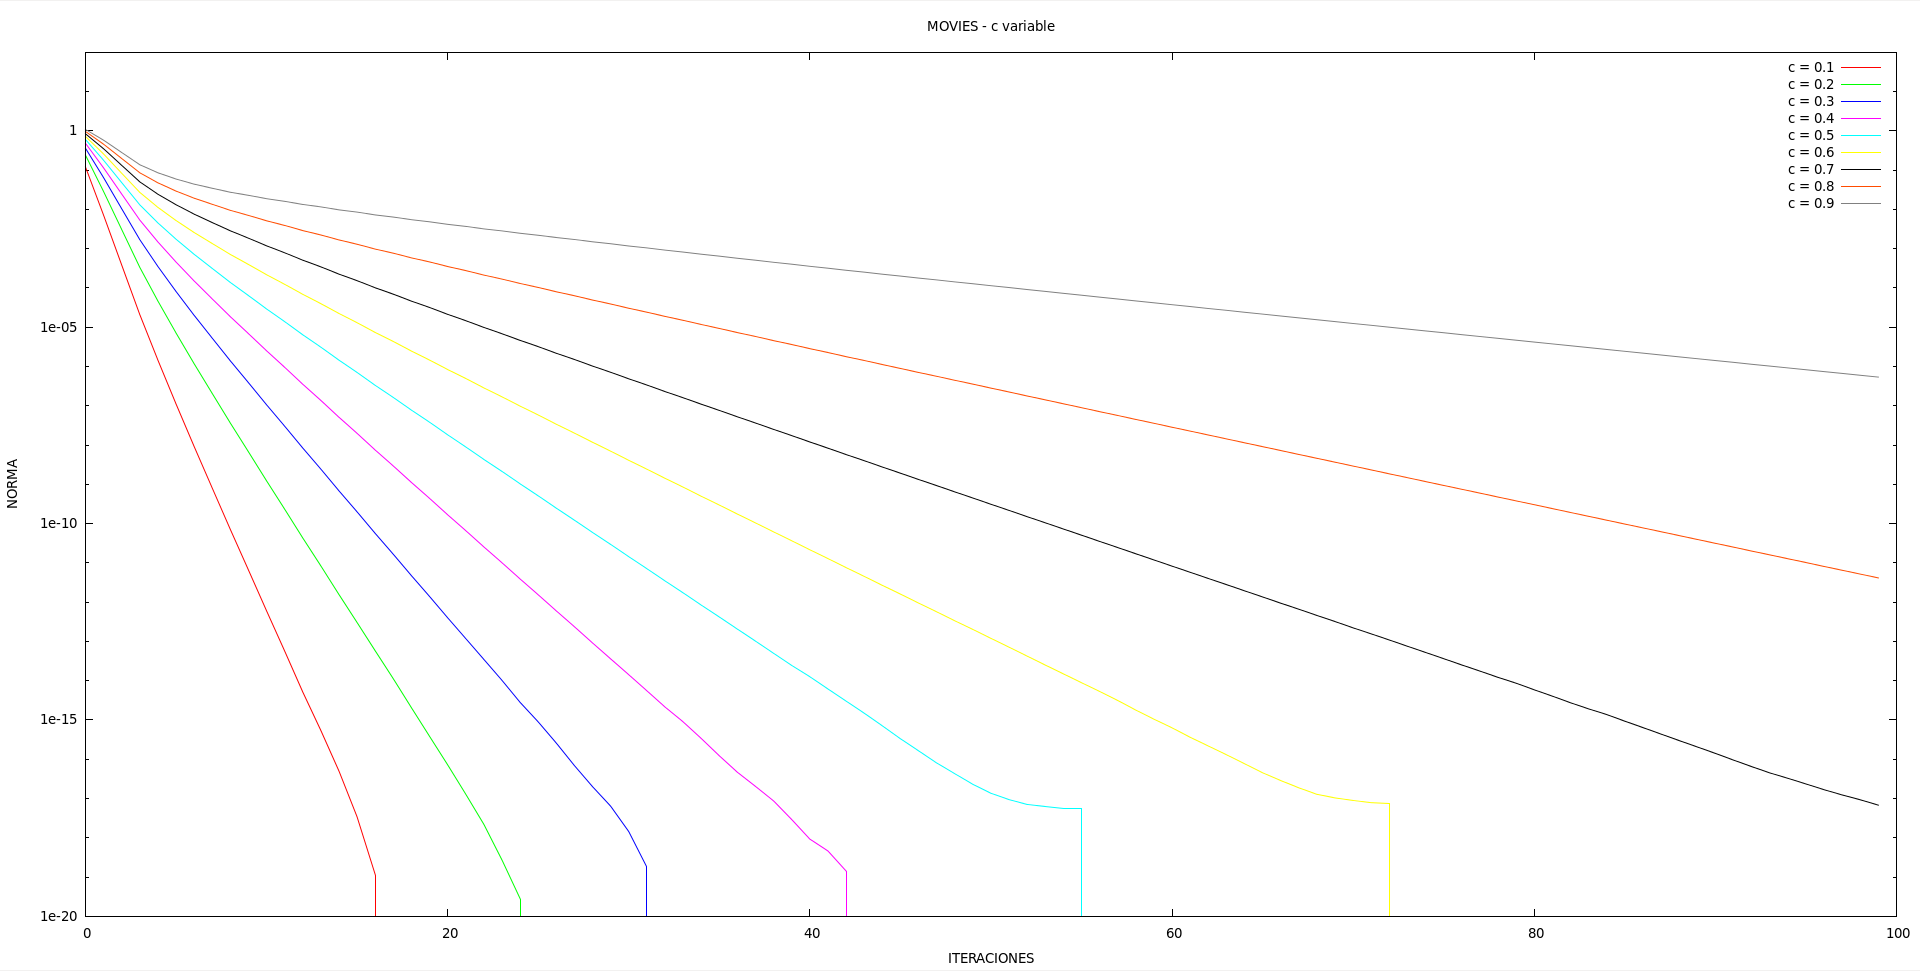
\includegraphics[width=1\textwidth]{imagenes/pagerank_norma.png}
\end{figure}

Claramente podemos notar que a medida que el C crece, el algoritmo toma más iteraciones en achicar la norma. Esto se debe a que el grado de aleatoriedad elimina el peso de la unión entre los sitios e indica una uniformidad en el comportamiento, entonces la matriz si bien estocástica ahora se encuentra distribuida esa suma $=$ 1 por columna en varias filas. Esto produce mayor cantidad de iteraciones en el método de la potencia$[1]$

\subsection{Comparación de Tiempos}
 
